\section{Elektronik}

\subsection{Robothand}
\begin{frame}
\begin{columns}
\column{0.6\textwidth}
[bild]
\column{0.4\textwidth}
\textbf{Komponenter}
\begin{itemize}
	\item Meccano-hand
	\item Arudino Due
	\item Bluetooth-enhet
	\item Trycksensorer
	\item Batteri eller AC/DC
	\item Work in progress
\end{itemize}
\end{columns}
\end{frame}


\subsection{Kontrollhandske}
\begin{frame}

\begin{columns}
\column{0.6\textwidth}
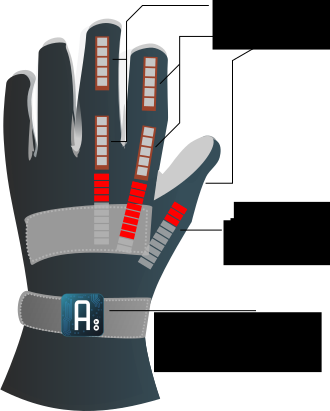
\includegraphics[height=\textheight]{../mittrapport/img/kontrollhandske}

\column{0.4\textwidth}
\textbf{Komponenter}
\begin{itemize}
	\item Handske
	\item Arduino Micro
	\item Bluetooth-enhet
	\item Flexsensorer
	\item Ledlampor
	\item Batteri
\end{itemize}
\end{columns}

\end{frame}



\subsection{Mikrokontroller}
\begin{frame}
\begin{block}{Arduino}
Populär bland hobbyelektronik, öppen mjukvara och hårdvara, många färdiga bibliotek.
\end{block}
\begin{columns}
\column{0.6\textwidth}
\textbf{Robothand}: Arduino Due
\begin{itemize}
	\item 32bitars ARM-arkitektur
	\item Måga in- och utportar
\end{itemize}

\textbf{Kontrollhandske}: Arduino Micro
\begin{itemize}
	\item Liten passform $(4.8\unit{cm} \times 1.77\unit{cm})$
	\item Låg strömförbrukning
	\item Tillräckligt med in- och utportar
\end{itemize}

\column{0.4\textwidth}
\includegraphics[width=\textwidth]{../mittrapport/img/arduino_micro}
\end{columns}
\end{frame}


\subsection{Trådlös överföring}
\begin{frame}
\begin{columns}
\column{0.7\textwidth}
\textbf{Bluetooth}
\begin{itemize}
	\item Standardiserat
	\item 20m räckvidd i ideala förhållande
	\item Säkerhet --- 128bit symmetrisk kryptering
	\item Integritet och paketförlust
	\item Bluetoothstacken i hårdvaran
	\item Överföringsprotokoll kan behöva definieras
\end{itemize}
\column{0.3\textwidth}
\centering

\includegraphics[width=0.5\textwidth]{../mittrapport/img/bluetooth} \\
\includegraphics[width=\textwidth]{../mittrapport/img/bluetooth_mate_silver}
\end{columns}
\end{frame}





